\documentclass[tikz,border=5pt]{standalone}
\usepackage{tikz}
\usetikzlibrary{arrows.meta, positioning}

\begin{document}
	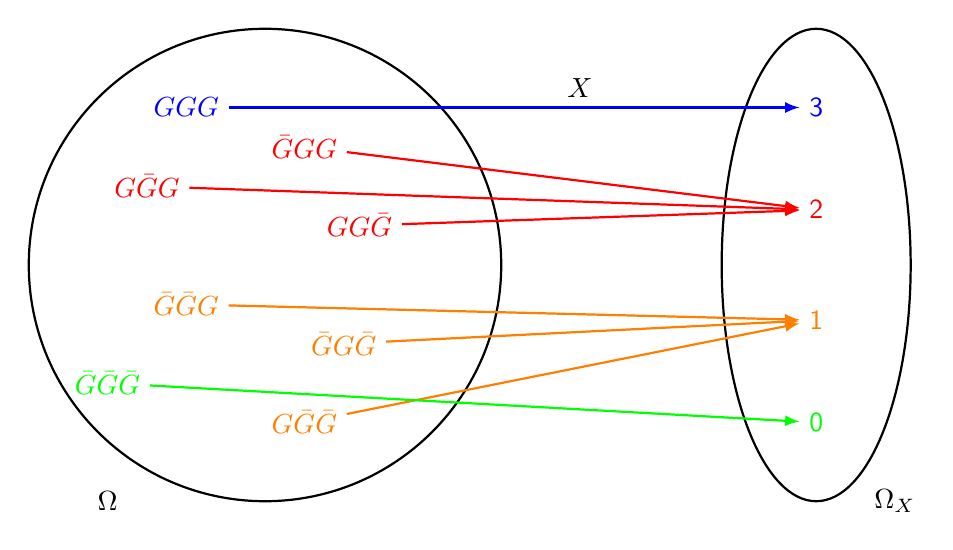
\begin{tikzpicture}[>=latex, font=\sffamily]
		
		% --- Espaço amostral (círculo à esquerda)
		\draw[thick] (0,0) circle (3cm);
		\node at (-2, -3) {$\Omega$};
		
		% Resultados dentro do espaço amostral
		\node[blue]  (GGG) at (-1,2) {$GGG$};
		\node[red]   (R1) at (0.5,1.5) {$\bar{G}GG$};
		\node[red]   (R2) at (-1.5,1) {$G\bar{G}G$};
		\node[red]   (R3) at (1.2,0.5) {$GG\bar{G}$};
		\node[orange](O1) at (-1,-0.5) {$\bar{G}\bar{G}G$};
		\node[orange](O2) at (1,-1) {$\bar{G}G\bar{G}$};
		\node[orange](O3) at (0.5,-2) {$G\bar{G}\bar{G}$};
		\node[green](PPP) at (-2,-1.5) {$\bar{G}\bar{G}\bar{G}$};
		
		% --- Conjunto dos valores possíveis de X
		\draw[thick] (7,0) ellipse (1.2cm and 3cm);
		\node at (8, -3) {$\Omega_X$};
		
		% Valores de X
		\node[blue]   (x3) at (7,2) {3};
		\node[red]    (x2) at (7,0.7) {2};
		\node[orange] (x1) at (7,-0.7) {1};
		\node[green] (x0) at (7,-2) {0};
		
		% --- Função aleatória X
		\node at (4,2.25) {$X$};
		
		% Setas
		\draw[->,blue,thick]   (GGG) -- (x3);
		\draw[->,red,thick]    (R1) -- (x2);
		\draw[->,red,thick]    (R2) -- (x2);
		\draw[->,red,thick]    (R3) -- (x2);
		\draw[->,orange,thick] (O1) -- (x1);
		\draw[->,orange,thick] (O2) -- (x1);
		\draw[->,orange,thick] (O3) -- (x1);
		\draw[->,green,thick] (PPP) -- (x0);
		
	\end{tikzpicture}
\end{document}
